\chapter{Dark matter overview}\label{chap:DarkMatterOverview}
\section{Evidence for dark matter}\label{sec:DMOverview/Evidence4DM}
In the latter part of the 19th century, astronomers began to propose the existence of non-luminous matter to account for the uneven distribution of stars observed in the night sky \cite{HistoryofDM}. One of the earliest quantitative attempts to estimate the presence of such "dark bodies" in the Milky Way was made by Lord Kelvin in 1904. Kelvin postulated that if stars in the Milky Way could be modelled analogously to particles in a gas, interacting primarily through gravity, then a relationship could be established between the size of the system and the velocity dispersion of its constituents \cite{Kelvin1904}. The term \textit{dark matter} (\textit{mati\`ere obscure}) was first introduced by Henri Poincar\`e in 1906. Based on Kelvin’s velocity dispersion calculations, Poincar\`e argued that the amount of dark matter was likely to be less than or equal to the amount of visible matter \cite{HPon}. In 1922, Jacobus Kapteyn developed one of the earliest models to quantitatively describe the size and structure of the Milky Way. His model characterized the stellar distribution as a flattened disk rotating about an axis aligned with the galactic pole. Kapteyn reached conclusions similar to those of Poincaré, asserting that the presence of significant quantities of unseen matter was improbable \cite{Kapteyn1922}.

While these early investigations did not yield definitive evidence for the existence of dark matter, they established a foundational framework upon which later studies would build more rigorous arguments for the presence of missing mass in the Galaxy.

\subsection{Virial theorem and the Coma Cluster}\label{sec:DMOverview/ViralTheorem}
The virial theorem is a fundamental result in classical mechanics that relates the average total kinetic energy $\langle T \rangle$ of a system to its average total potential energy $\langle U \rangle$. The theorem can be used to estimate the mass of a galaxy cluster through the following approximation:
\begin{equation}
\begin{split}
2\langle T \rangle + \langle U \rangle = 0, \\
Nm\langle v^2\rangle - \frac{3}{5}\frac{GN^2m^2}{R}=0,\\
Nm=\frac{5R\langle v_r^2 \rangle}{G},\\
\end{split}
\label{eq:DMOverview/virial}
\end{equation}
where $N$ is the estimate number of galaxies in the cluster, $M$ is the observed seller mass of the galaxies in the cluster, $v_r$ is the radial velocities, and $R$ is the radius of the cluster.
In 1933, Fritz Zwicky applied the virial theorem to the Coma Cluster of galaxies \cite{Zwicky1933}. He measured the radial velocities of galaxies within the cluster and estimated their velocity dispersion. When he used the virial theorem to estimate the total mass required to gravitationally bind the system, he estimated the minimum mass of the galaxies in the cluster to be $M=4\times 10^{10}M_{\odot}$, where $M_{\odot}$ is one solar mass. With an average velocity dispersion observed to be approximately 1000~kms$^{-1}$, the mass-to-light ratio that was far too large to be accounted for by visible matter alone \cite{HistoryofDM}. Zwicky’s analysis revealed that the total mass inferred from the virial theorem was roughly 400 times greater than what could be explained by the luminous matter. To resolve this discrepancy, he proposed the existence of a substantial amount of unseen mass, which he referred to as \textit{dunkle Materie}, or “dark matter” \cite{Zwicky1933}.

\subsection{Galaxy rotation curves}\label{sec:DMOverview/RotationCurves}
A galaxy rotation curve describes the variation of orbital velocity of stars and gas as a function of their radial distance from the galactic centre. Under the assumption that a galaxy's mass is distributed entirely within its luminous matter, one would expect the mass to be concentrated primarily near the galactic centre. Therefore, the orbital velocity of objects situated at large radii should decrease with distance, according a Keplerian dynamics given by:
\begin{equation}
v(r) \propto \frac{1}{\sqrt{r}},
\end{equation}
where $v(r)$ is the orbital velocity and $r$ is the radial distance from the galactic centre.
In 1978, Vera C. Rubin \textit{et al.}\cite{Rubin} analysed the hydrogen spectra from a sample of ten high-luminosity spiral galaxies. By measuring the Doppler shift of the 21~cm line in the hydrogen spectra, they were able to determine the rotation velocities of gas and stars across a range of galactic radii. Rubin found that the rotation curves of these galaxies remained approximately constant, whilst the orbital velocities stayed constant, even at large radii. This observation was inconsistent with the mass inferred from visible matter alone and the expectations resulting from applied Keplerian dynamics.
A representative velocity profile for the galaxy NGC 6503 is shown in \autoref{fig:NGC6503}. The high orbital velocities at large radii suggests that a significant portion of galactic mass must be distributed well beyond the visible edge. This led to the hypothesis of a surrounding, non-luminous mass component, commonly referred to as a dark matter ``halo'' that provides the additional gravitational influence required to maintain the observed rotation velocities. The presence of such halo could explain the observed phenomena.
\begin{figure}[ht]
	\centering
	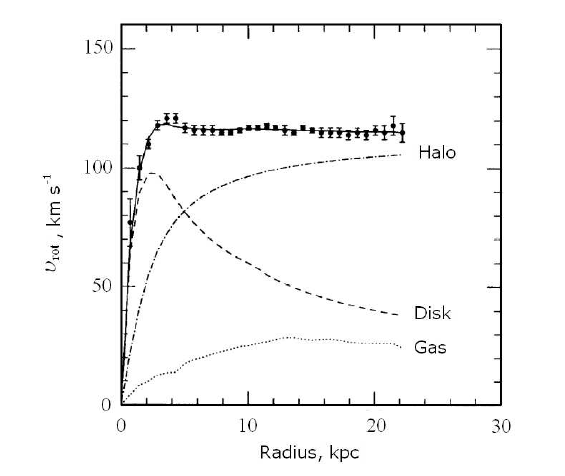
\includegraphics[width = 0.6\textwidth]{figures/DMOverview/NGC_6503.png}
	\caption[Galactic rotation curve for NGC 6503.]{Galactic rotation curve for NGC 6503. The dotted and dashed lines represents where the data should lie if Keplerian dynamics are obeyed. The dot-dashed line indicates the dark matter `halo' contribution needed for the function to fit the data \cite{Freese2009}.}
	\label{fig:NGC6503}
\end{figure}
\subsection{Gravitational lensing}\label{sec:DMOverview/GravLens}
The observed effect of gravitational lensing can be used to infer the total mass of astronomical objects. An example of the effect gravitational lensing has on light from a distant galaxy is shown in \autoref{fig:DMOverview/GravLens}. The effect was first described theoretically by Albert Einstein in 1936 \cite{GravLens}. The effect occurs when a massive object (lensing object) is situated in the line of sight between a distant source and an observer. Due to the gravitational field of the lensing object, light from the source deflects from its path resulting in observable distortions such as magnification, image splitting, or the formation of arcs and rings.
When the lensing is strong enough to produce multiple images or highly distorted arcs, it is referred to as \textit{strong gravitational lensing}. An example of such an effect is shown in \autoref{fig:DMOverview/StrongGravLens}. The degree of light deflection depends on the gravitational potential of the lensing object, which can be reconstructed by analysing the extent and geometry of the observed distortions \cite{Young2016}.

The mass of the lensing object in the line of sight is compared with that of the observed baryonic matter (stars, dust and gas), and the existence of dark matter is inferred to explain the discrepancy between the visible mass and lensing mass. 
\begin{figure}[ht!]
	\centering
	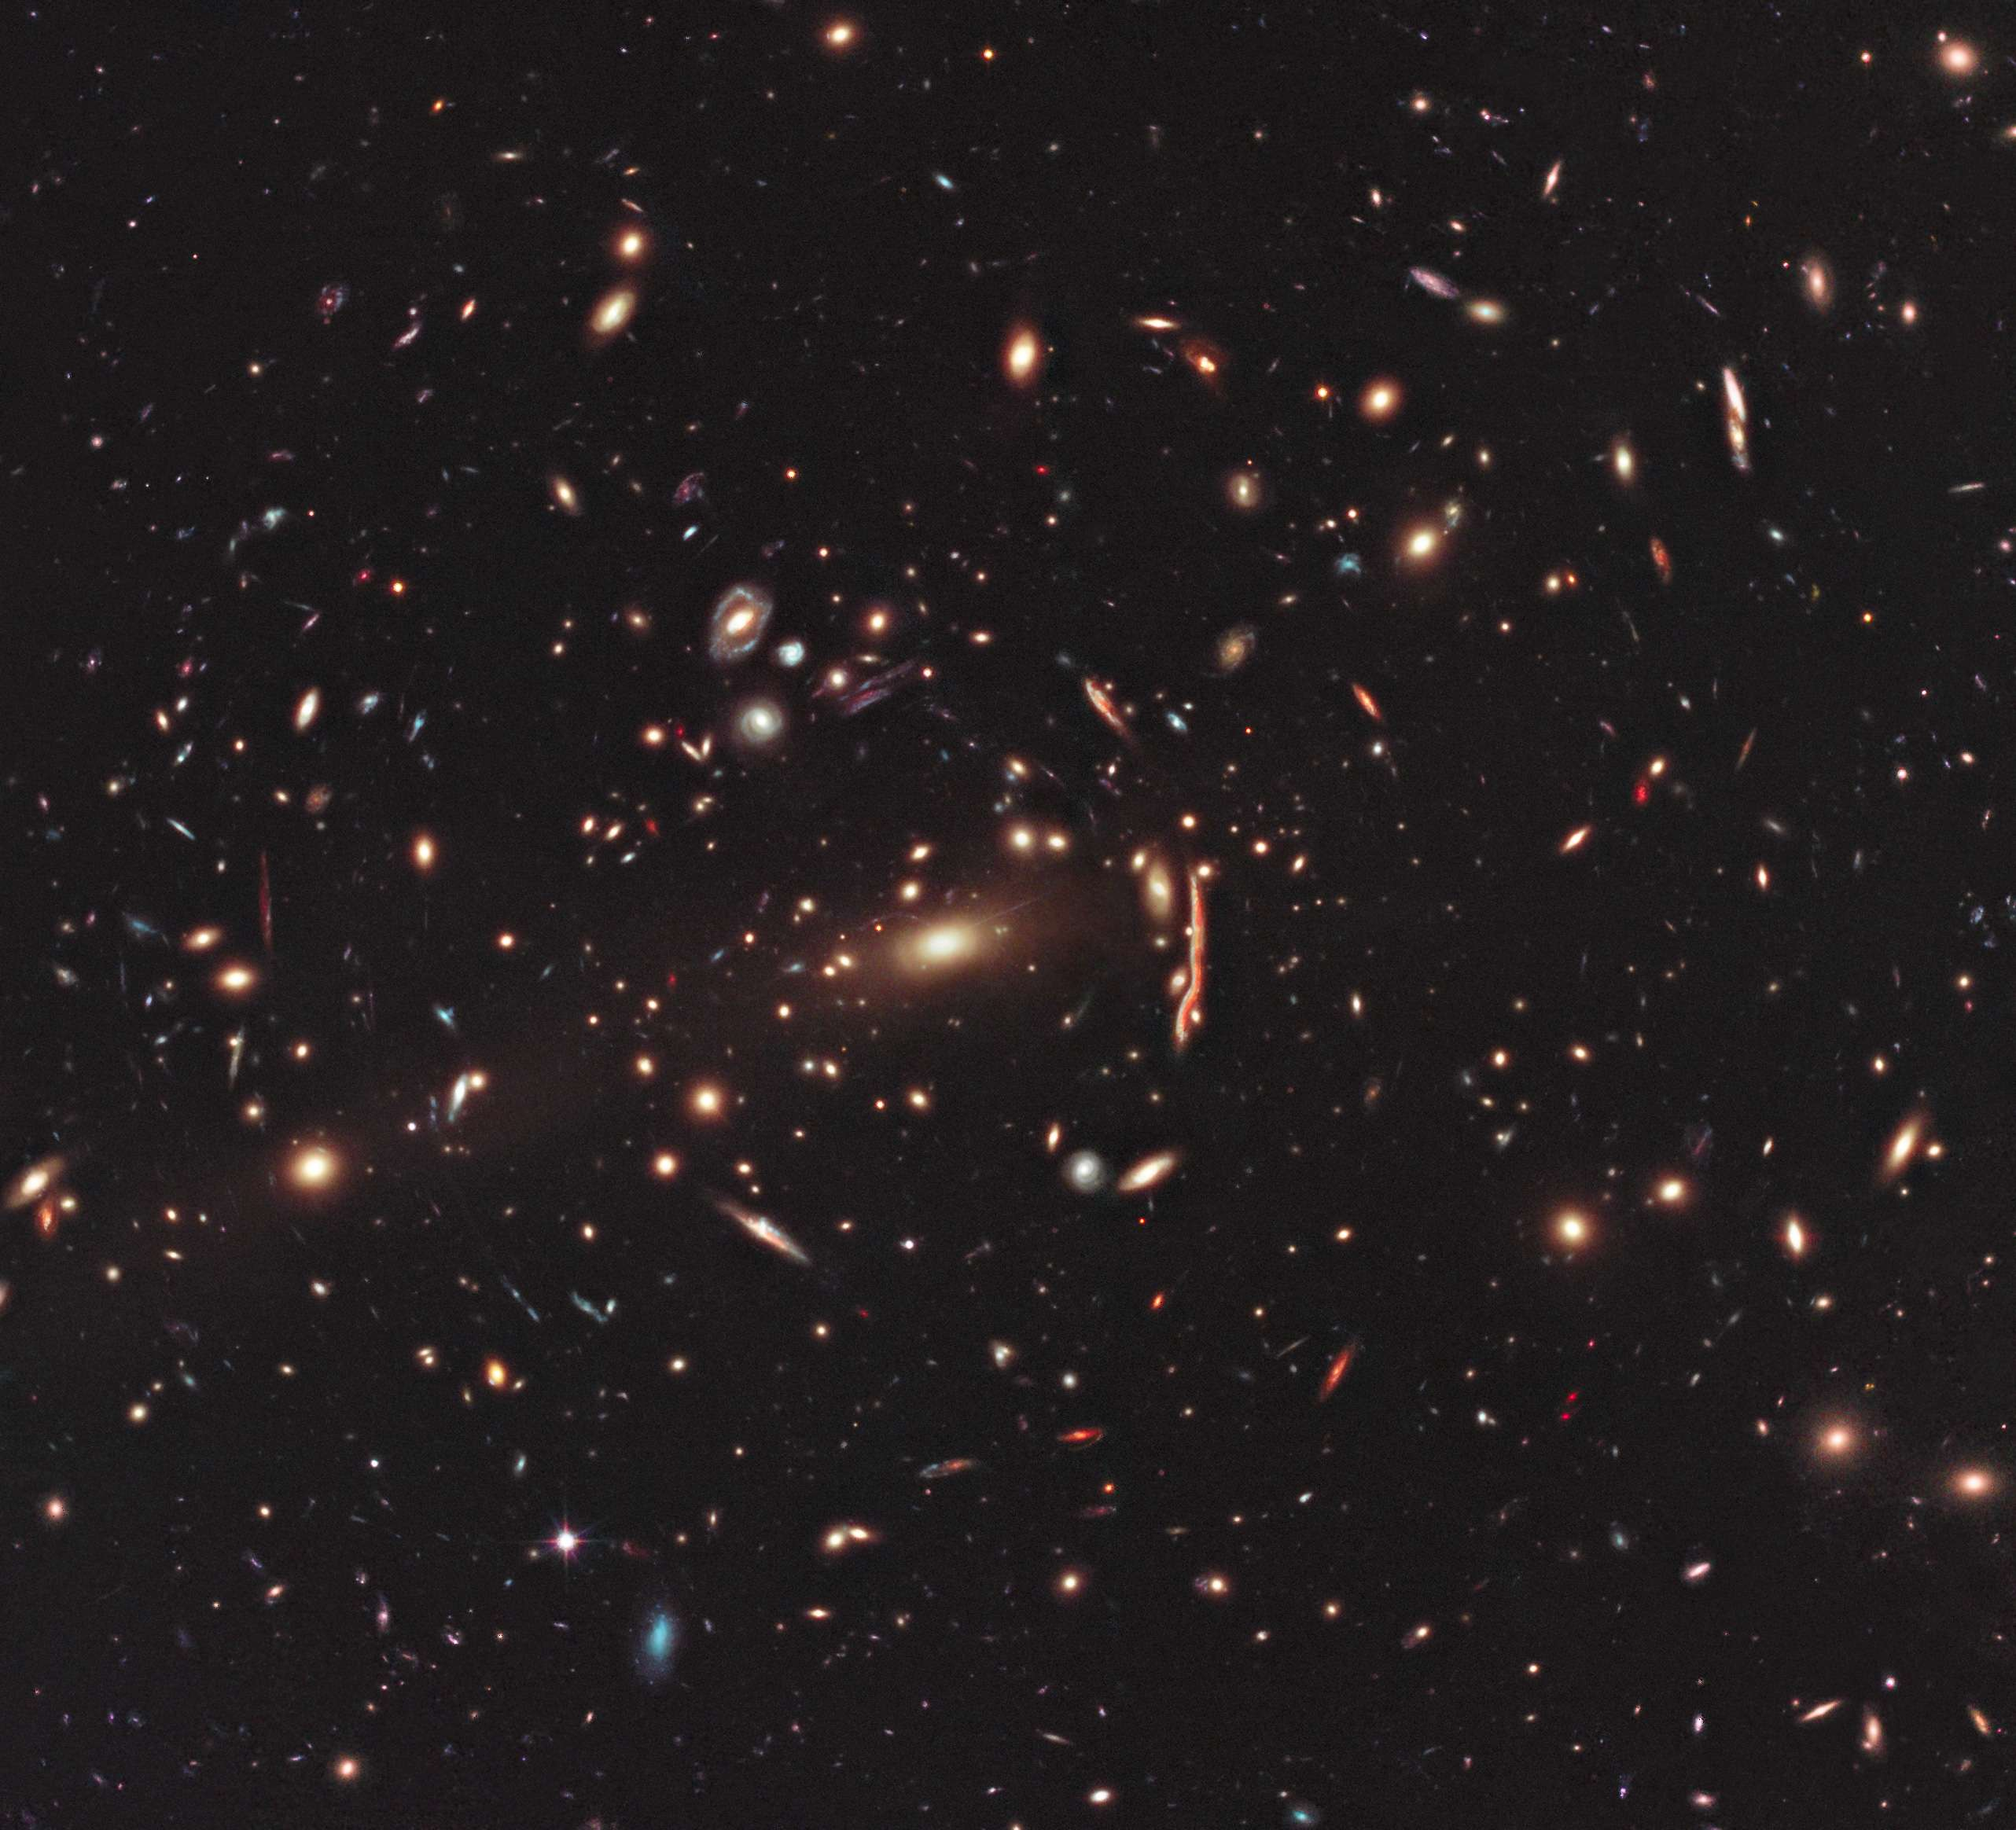
\includegraphics[width=0.6\textwidth]{figures/DMOverview/GravLensIm.jpg}
	\caption[Gravitational lensing by the galaxy cluster MACS J1206.2-0842s.]{Gravitational lensing by the galaxy cluster MACS J1206.2-0842s \cite{GravLensPicture}. The image was taken by the NASA/ESA Hubble Space Telescope, this galaxy is one of 25 clusters being studied as part of the Cluster Lensing and Supernova survey with Hubble programme.}
	\label{fig:DMOverview/GravLens}
\end{figure}
\begin{figure}[ht!]
	\centering
	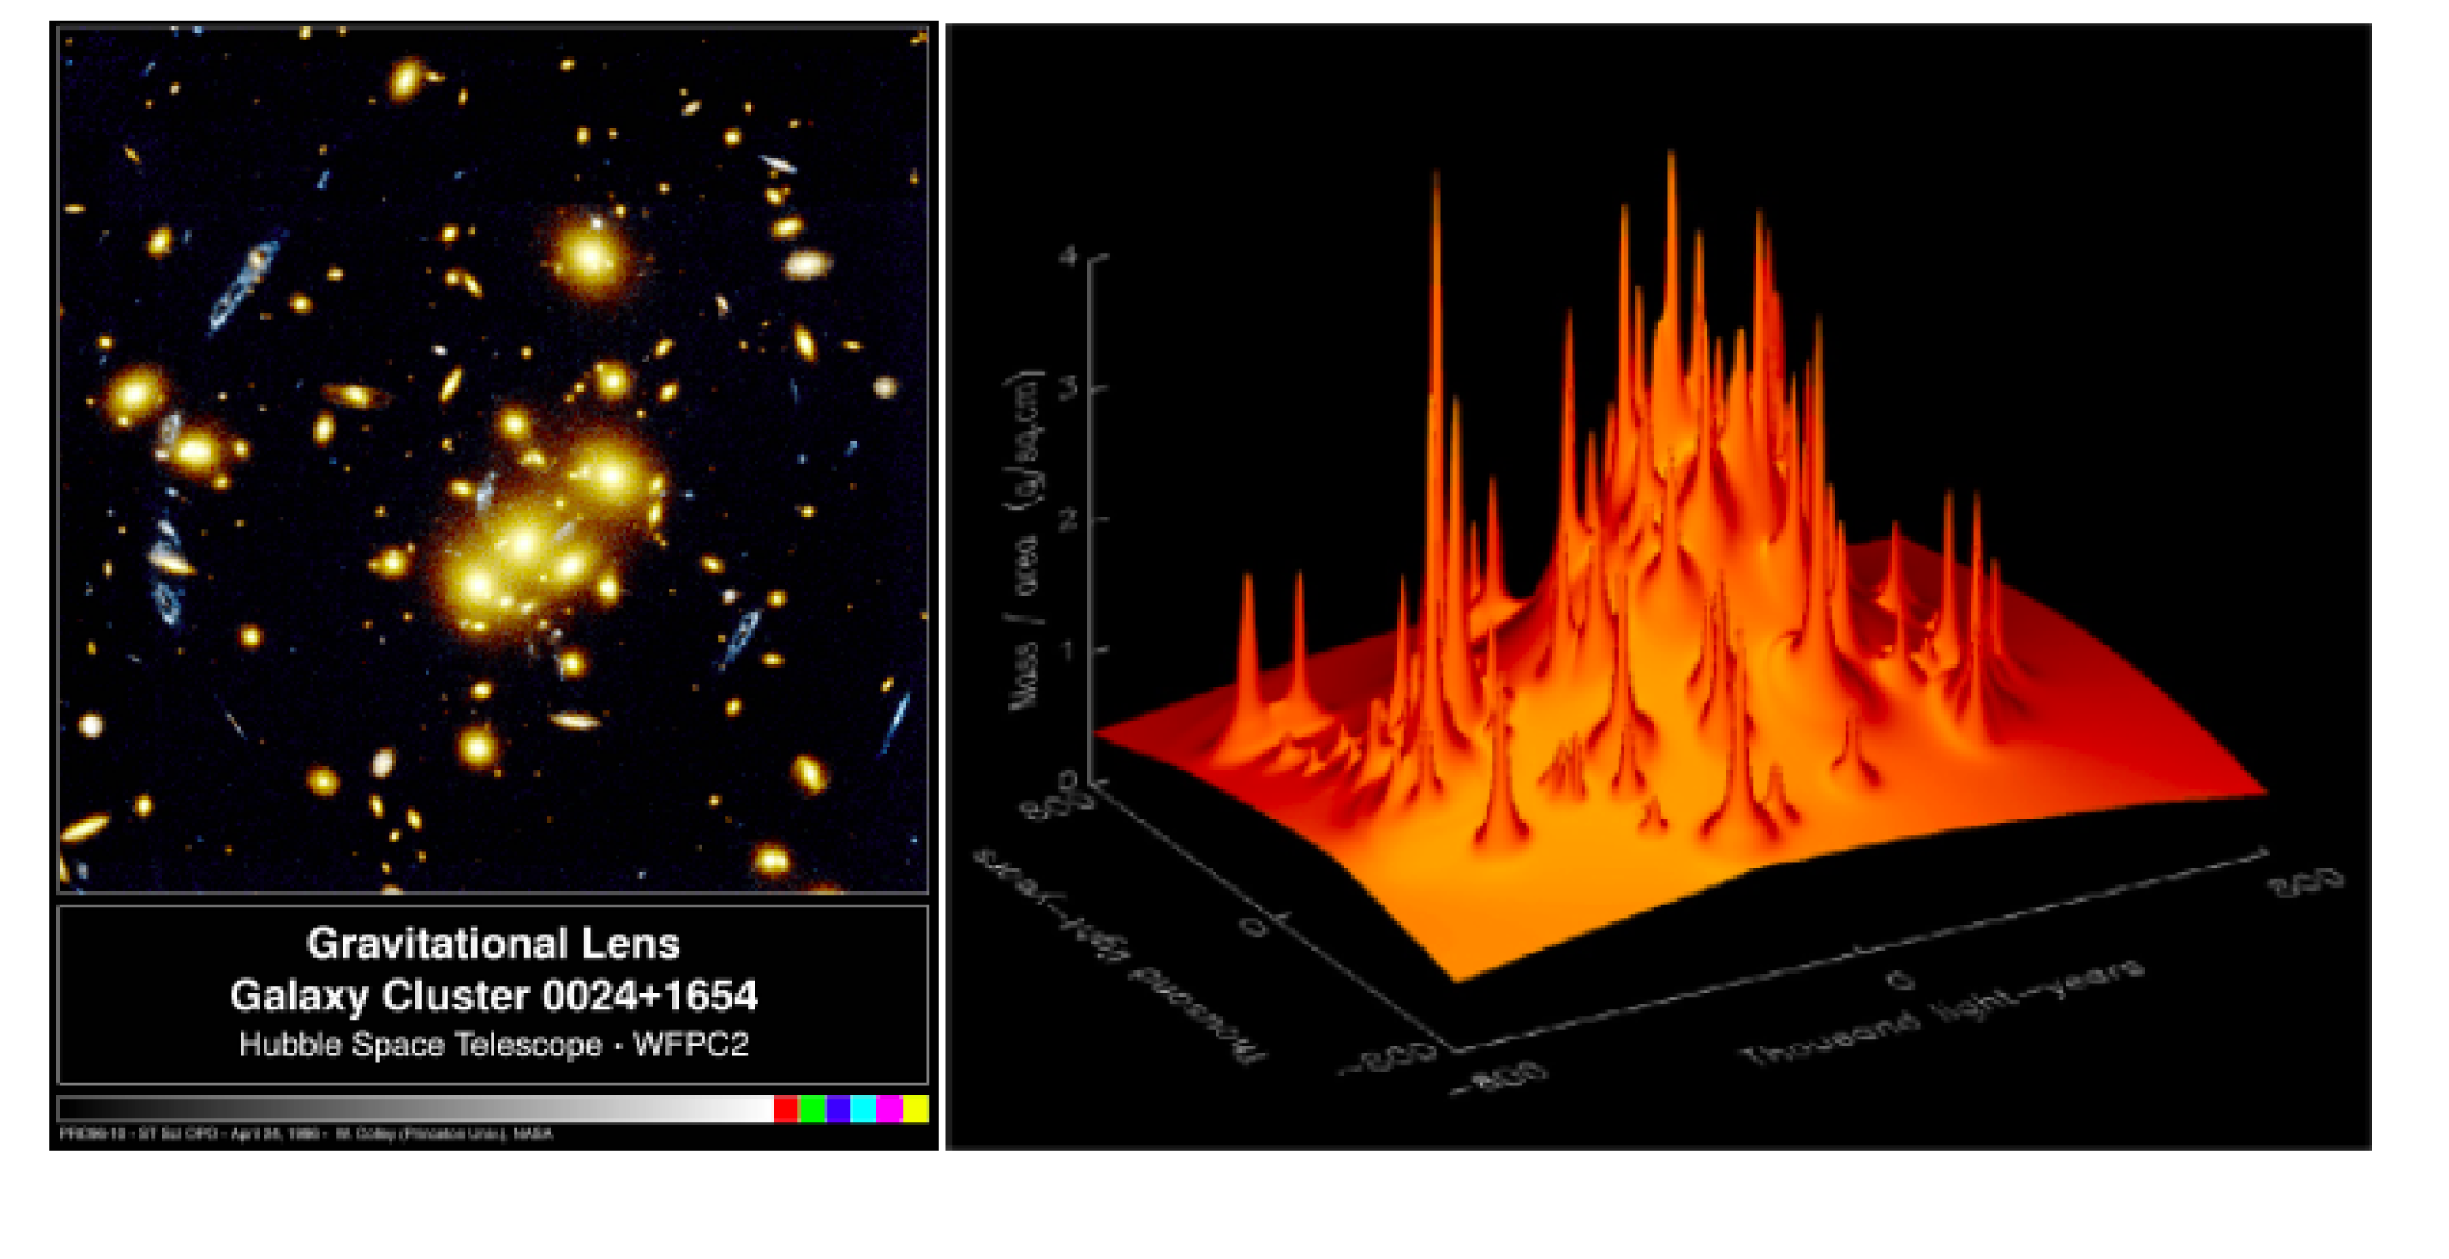
\includegraphics[width=0.8\textwidth]{figures/DMOverview/Strong_Grav_lens.png}
	\caption[\textbf{Left:} Effects of gravitational lensing on multiple galaxies. \textbf{Right:} Reconstruction of gravitational lensing effects.]{\textbf{Left:} An image from the Hubble Space Telescope where the foreground cluster of galaxies gravitationally lenses the blue background galaxy. \textbf{Right:} A reconstruction of gravitational lensing by galaxy cluster. Baryonic matter within the cluster are represented by the sharp spikes and the smooth background component corresponds to some non-visible mass \cite{Freese2009}.}
	\label{fig:DMOverview/StrongGravLens}
\end{figure}
\subsubsection{The Bullet Cluster}\label{sec:DMOverview/BulletCluster}
Observations of the Bullet Cluster (1E 0657–56) made by the Hubble Space Telescope and the Chandra X-ray Observatory provides evidence towards the existence of dark matter using gravitational lensing.
The Bullet Cluster consists of two galaxy clusters which have collided and are now moving apart. A composite image of the cluster can be seen in \autoref{fig:DMOverview/BulletComp}, where colour overlays represent the distribution of both luminous and total mass components. The blue regions in the image highlight the total mass distribution derived from gravitational lensing measurements, while the pink regions represent the hot, X-ray-emitting gas that contains the majority of the baryonic matter, such as gas and dust. Analysis of the X-ray data found that as the two clusters passed through one another, their gaseous components interacted strongly, colliding, slowing down, and heating up, thus producing intense X-ray emissions. Whereas measurements made using gravitational lensing indicated that the majority of the non-luminous portion of mass continued without disruption. The lensing mass peaks of the colliding clusters were compared with the X-ray peaks and an offset was found \cite{Clowe_2004}. The offset found between the peaks is considered strong evidence towards the presence of dark matter within the two colliding clusters. Clowe \textit{et al.} applied Modified Theories of Newtonian Dynamics (MOND) to the results to explain the Bullet Cluster formation but were unable to fully explain the effect where the dark matter component in the regime was equal to the baryonic mass in the system \cite{Clowe2006}. Therefore the presence of dark matter in the cluster still holds true. Thus the Bullet Cluster observations remain as the ``smoking gun'' in the pieces of evidence which support the existence of dark matter in the Universe.
\begin{figure}[ht!]
	\centering
	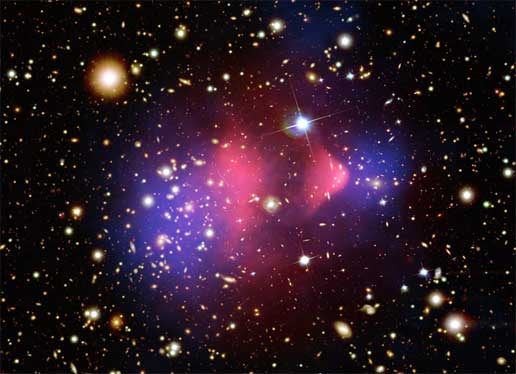
\includegraphics[width=0.8\textwidth]{figures/DMOverview/Bullet_cluster.jpg}
	\caption[An image of the Bullet Cluster highlighting the distribution of mass within the two colliding clusters.]{An image of the Bullet Cluster highlighting the distribution of mass within the two colliding clusters. The pink region indicate where the majority of the baryonic matter is situated formed from X-ray analysis. The blue regions are produced from gravitational micro-lensing measurements highlighting where the total mass of colliding clusters is located \cite{chandra}.}
	\label{fig:DMOverview/BulletComp}
\end{figure}
\section{The Cosmic Microwave Background}\label{sec:DMOverview/CMB}
The Cosmic Microwave Background (CMB) was first predicted by Ralph Alpher and Robert Herman in 1948 \cite{CMBprediction}, and subsequently discovered by Arno Penzias Robert Woodrow Wilson in 1964 \cite{CMBDisco}. The CMB is relic radiation released after the Big Bang during the recombination epoch. The Universe was filled with an extremely dense, hot-plasma of photons and charge particles. There was an initial rapid expansion of the Universe over 380,000 years until the rate of expansion decreased as the temperature cooled approaching the recombination epoch \cite{DMPrimer}. During this time neutral particles were formed which don't interact with photons. The photons which were once coupled to charged particles in the plasma state were able to stream freely through the Universe. The CMB is the result of the photons released during this ``last scattering'' \cite{Cirelli:2024ssz}.

The CMB is not completely homogeneous and isotropic, however it can still be viewed as a black body spectrum with a temperature of $(2.726\pm0.001)$~K \cite{Fixsen_2009}. Fluctuations in the relic density after recombination are echoed in the relic temperature when gravity began to dominate matter. These variations are known as the CMB anisotropy. As a result, the CMB carries an imprint of the presence of dark matter which are reflected in acoustic oscillations in the plasma where gravity provided the restoring force. The main observable is the CMB power spectrum shown in \autoref{fig:DMOverview/CMBPowerSpec} which is obtained by performing a spherical Fourier transform of the photon temperature field shown in \autoref{fig:DMOverview/CMBImg}, and then computing the variance by averaging over the $2l+1$ orientations for each value of the angular momentum $l$ \cite{Cirelli:2024ssz}. The variations are compared to predictions of inflationary Big Bang cosmology which infers information on the contents of the Universe. More precisely, the CMB peaks are due to acoustic oscillations of the baryon/photon fluid. The positions and amplitudes of the peaks represent the relative amount of dark matter with respect to normal matter, where only the latter undergo acoustic oscillations. Global fits to the spectrum find that these oscillations and additional cosmological observations can be well produced by the Standard Model of cosmology which includes dark matter ($\Lambda \text{CDM}$. The x-axis in \autoref{fig:DMOverview/CMBPowerSpec} is a rank of the multiple moment which is inversely proportional to the angular coverage of the sky where,
\begin{equation}
    l \approx\frac{180\degree}{\theta_{res}(degrees)},
\end{equation}
which is treated as a continuous variable \cite{Young2016}. The first peak t $l=200$ infers the total energy-matter density ratio to be $\Omega_{total}=1$. The size and location of the peak relates to the ``flat'' shape of the universe. The second peak centred at $l\approx500$ informs how much baryonic matter is present in the universe. And the third peak at $l\approx700$ describes both the baryonic and dark matter components, where the difference between the second and third peak provides information of the density of dark matter in the early universe \cite{Young2016}.
\begin{figure}[!ht]
     \centering
     \begin{subfigure}{0.47\textwidth}
         \centering
         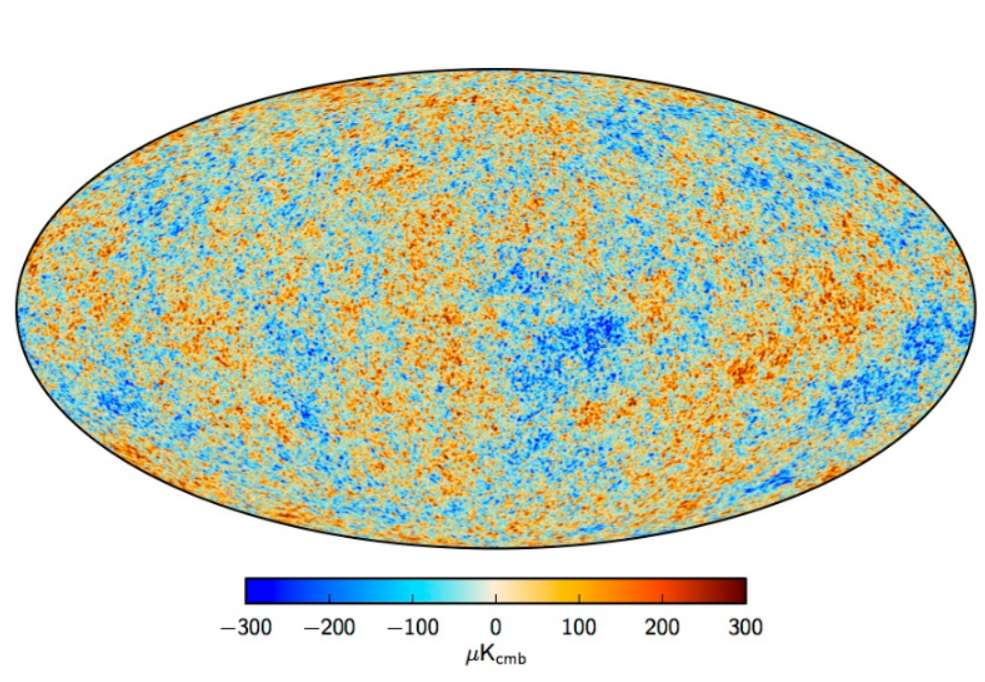
\includegraphics[width=\textwidth]{figures/DMOverview/CMBImg.png}
         \caption{}
         \label{fig:DMOverview/CMBImg}
     \end{subfigure}
     \hfill
     \begin{subfigure}{0.47\textwidth}
         \centering
         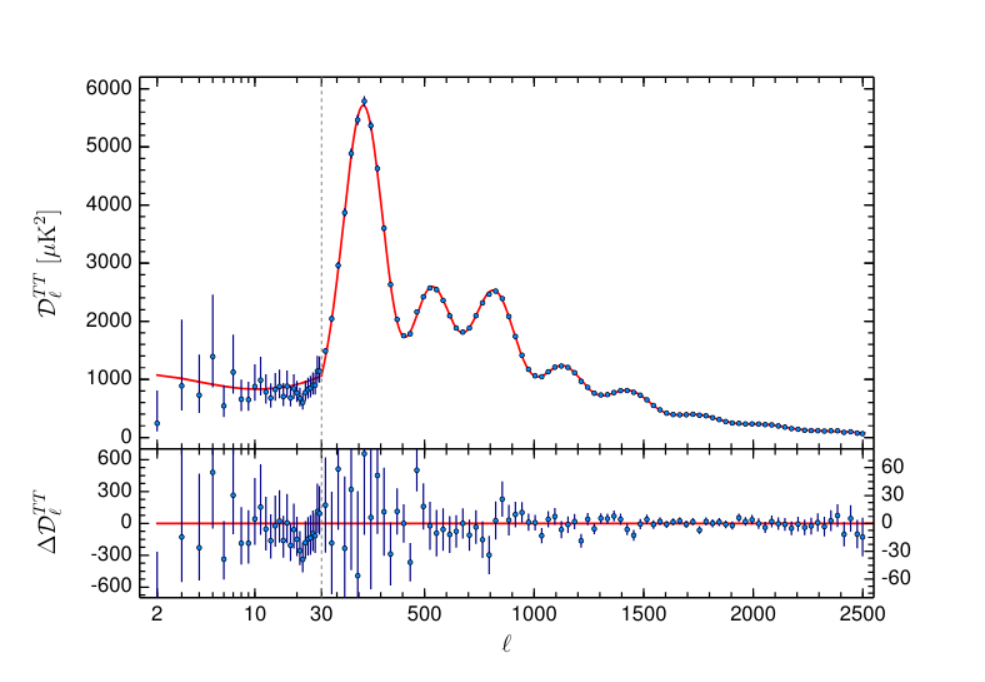
\includegraphics[width=\textwidth]{figures/DMOverview/CMBPS.png}
         \caption{}
         \label{fig:DMOverview/CMBPowerSpec}
     \end{subfigure}
     \caption{The power spectrum of the CMB acoustic peaks (right) is extracted from the map of temperature anisotropies (left). Figures reprinted from Ref.~\cite{Cirelli:2024ssz}.}
     \label{fig:DMOverview/CMB}
\end{figure}
\subsection{$\Lambda$CDM model}\label{sec:DMOverview/LambdaCDM}
Blah

\section{Avoiding dark matter}\label{sec:DMOverview/AvoidDM}

\subsection{Modification of Newtonian dynamics}\label{sec:DMOverview/MOND}

\subsection{MACHOs}\label{sec:DMOverview/MACHOs}

\section{Possible candidates for dark matter}\label{sec:DMOverview/Candidates4DM}

\subsection{WIMPs}\label{sec:DMOverview/WIMPs}

\subsection{Sterile neutrinos}\label{sec:DMOverview/Neutrinos}

\subsection{Axions}\label{sec:DMOverview/Axions}

\section{Searching for dark matter}\label{sec:DMOverview/DetectionOfDM}

\subsection{Indirect detection of dark matter}\label{sec:DMOverview/IndirectDM}

\subsection{Dark matter production at colliders}\label{sec:DMOverview/DMProdColliders}

\subsection{Direct detection of dark matter}\label{sec:DMOverview/DirectDetection}

\section{Current status for dark matter searches}\label{sec:DMOverview/DMCurrentStatus}